\section{Proposed Approach}
\label{sec:proposed_approach}
% This section introduces the Push-Pop model and designs the TTR algorithm in Push-Pop model for blockchain transaction tracking.
This section introduces the architecture, implementation, and theoretical analysis of TRacer.

\subsection{Architecture Overview}
TRacer consists of three main modules including graph construction, graph expansion, and local community detection. Each module is described as follows:
\begin{itemize}
\item \textbf{Graph construction}: This module models the money transfer relationships between accounts as directed, weighted, temporal, and multi-relationship graphs.
% in which the nodes and the edges represent the accounts and the transactions in the blockchain, respectively.
\item \textbf{Graph expansion}: Since the blockchain data contains billions of transactions which is too large for common graph algorithms, this module aims to find a relevant subgraph from a risky source. The module contains four operations: \textit{\textbf{Expand}} collects all edges related to a given node, \textit{\textbf{Push}} merges the collected edges to the subgraph, \textit{\textbf{Rank}} computes the relevance of nodes in the subgraph to the source, and \textit{\textbf{Pop}} selects a node for expanding.
The graph expansion process terminates when the end condition is met.
\item \textbf{Local community detection}: This module \textit{\textbf{Extract}}s a local community of the source node from the expended subgraph, in which nodes have higher relevance to the source than nodes out of the community.
\end{itemize}

\subsection{Graph construction}
Since there are multiple types of tokens in account-based blockchain trading systems, we formulate the money transfer relationships among accounts into a directed, weighted, temporal, and multi-relationship graph $G=(V, E)$, where $V$ is the node set representing accounts, $E$ is the edge set representing the token transfer relationships.
% with $\varphi_E: E\rightarrow\{{\rm token \ types}\}$ for edge-type mapping
% , and $X$ denotes the set of attributes attached to edges including transaction hash (unique to the corresponding external transaction), amount, timestamp, and token symbol. 
An edge $e=(u,v,w,t,b,h)$ denotes that account $u$ transfer $w$ units token $b$ to account $v$ at timestamp $t$ with a transaction hash $h$. We define mapping functions $f_{src}$, $f_{tgt}$, $f_{amt}$, $f_{ts}$, and $f_{sym}$ to map each edge to its source, target, amount, timestamp, and token type respectively. There are multiple types of edges indicating the transfer relationships of different tokens.

In addition, many blockchain services such as decentralized exchanges act as the intermediary for token swap. 
To reveal the token flows after users interact with these services, we categorize the money transfer relationships into two patterns, namely \textbf{Xfer} and \textbf{Swap}.
As shown in Figure \ref{fig:Xfer}, accounts send or receive tokens through the Xfer pattern, and the related DeFi actions \cite{wu2021defiranger} in this pattern include: 1) \textbf{\textit{transfer}}: An account sends an amount of token to another account, 2) \textbf{\textit{minting}}: A token contract mints an amount of token to an account, and 3) \textbf{\textit{burning}}: An account burns an amount of token.
While accounts exchange tokens for other kinds of tokens through the Swap pattern as shown in Figure \ref{fig:Swap}, including three related DeFi actions: 1) \textbf{\textit{add liquidity}}: An account deposits an amount of token to a DeFi app, and receives a certain amount of Liquidity Provider (LP) token back, 2) \textbf{\textit{remove liquidity}}: An account sends an amount of LP token to a DeFi app for destroying and gets a certain amount of other tokens back, and 3) \textbf{\textit{trade}}: An account sells an amount of token A in a DeFi app for a certain amount of token B. We identify the transaction relationships involving both the sending of tokens and the receiving of another kind of tokens with the same hash as the relationships in the Swap pattern, and otherwise as the relationships in the Xfer pattern. 
% In this way, we define the pattern mapping for the edges in the transaction graph:
% \begin{equation}
%     P: E \rightarrow \{Xfer, Swap\}.
% \end{equation}

% In addition, considering the token transfer, there are two types of patterns for a transaction in TRacer, namely \textbf{Xfer} and \textbf{Swap}.
% A transaction is recognized as Swap if the transactions with the same transaction hash ensure an account sending and receiving tokens at the same time, otherwise Xfer.
% These two patterns are summarized from the transaction actions defined by token contracts and DeFi DApps. 
% Several main actions \cite{wu2021defiranger} are listed below:
% \begin{itemize}
%     \item \textbf{Transfer}: An account sends an amount of token to another account.
%     \item \textbf{Minting}: A token contract sends an amount of minted token to an account. 
%     \item \textbf{Burning}: An account sends an amount of token to a token contract for destroying.
%     \item \textbf{Add Liquidity}: An account deposits an amount of token to the DeFi app, which also sends its an amount of Liquidity Provider (LP) token to the account.
%     \item \textbf{Remove Liquidity}: An account sends an amount of LP token to a DeFi app for destroying, and the account gets a number of other tokens back.
%     \item \textbf{Trade}: An account sells an amount of token A in a DeFi app for a certain amount of token B.
% \end{itemize}

\begin{figure}[t]
    \centering
    \subfigure[The Xfer pattern]{
    
\includegraphics[width=0.3\linewidth]{figures/Xfer.png}
    \label{fig:Xfer}
    }
    \subfigure[The Swap pattern] {
    
\includegraphics[width=0.35\linewidth]{figures/Swap.png}
    \label{fig:Swap}
    }
    \caption{(a) Xfer: Sending or receiving tokens.
    % Transaction actions in this pattern include transfer, minting, and destroying. 
    (b) Swap: Exchanging tokens for other kinds of tokens. 
    % Transaction actions in this pattern include add liquidity, remove liquidity, and trade.
    }
\end{figure}

\subsection{Graph Expansion}
The graph expansion module aims to obtain a relevant subgraph expanded from a given seed via iterating four operations shown in Figure \ref{fig:TRacer}. In what follows, we introduce the design of these four operations.
\subsubsection{\textit{Push} and \textit{Rank}: Transaction Tracing Rank}
The \textit{Push} operation merges the expanded edges to the subgraph in each iteration. While \textit{Rank} calculates the relevance of nodes in the subgraph to the source.
% While Rank is the core operation of graph extension in TRace, which determines the rules for calculating the relevance of nodes to the source node in the subgraph.

We introduce APPR to calculate the node relevance. 
More specifically, the Rank operation executes the local push procedure for the incremental update of node relevance.
% Especially, according to some characteristics of the transaction graph in account-based blockchain, we design a novel local push procedure. 
% The relevance computed using this novel local push procedure is named \textbf{Transaction Tracing Rank} (TTR).
Based on the characteristics of blockchain transaction graph in account-based blockchains, we propose a novel local push algorithm named \textbf{\underline{T}ransaction \underline{T}racing \underline{R}ank (TTR)} to compute the node relevance in blockchain transaction graph. We develop four local push strategies in TTR, namely \textbf{tracing tendency, weighted pollution, temporal reasoning, and token redirection}. We use $r_s(u,t,b)$ to denote the residual of node $u$ brought from token $b \in B$ at timestamp $t \in \Gamma$, where $\Gamma$ is the timestamp set and $B$ is the token symbol set in the subgraph.
% In the local push procedure of TTR, the edge attributes of time and token symbol need to be considered, thus we use $r_s(u,t,b)$ to denote the residual attached with a timestamp $t \in \Gamma$ and a token symbol $b \in B$ in the node $u$, where $\Gamma$ is a set of timestamps, and $B$ is a set of token symbols.
% % the residual is stored by a dictionary structure with the definition below:
% % \begin{equation}
% %     r_s: V \times \Gamma \times B \rightarrow \mathbb{R},
% %     \label{req:residual_mapping}
% % \end{equation}
% % where $V$ denotes a set of nodes, $\Gamma$ denotes a set of timestamps, and $B$ denotes a set of token symbols.
In this way, the local push procedure in TTR is described as Algorithm \ref{alg:ttr_local_push}. During initialization, a part of the residual of node $u$ is transformed into the relevance (line 1). Moreover, other parts of the residual are pushed to the neighbors according to the four strategies.
% 伪代码备份
% \begin{algorithm}[t]
%     \caption{TTR local push}
%     \label{alg:ttr_local_push}
%     \begin{algorithmic}[1]
%         \REQUIRE Node $u$, edges $E(u)$ related to $u$, rank $\bm{p}_s$, residual $r_s$, timestamp set $\Gamma$, and token symbol set $B$.
%         \ENSURE The updated $\bm{p}_s$ and $r_s$.
%         %% 自环
%         \STATE $\bm{p}_s(u) = \bm{p}_s(u) + \alpha \sum\limits_{b \in B}\sum\limits_{t \in \Gamma}r_s(u,t,b)$
%         \STATE $r'_s(u,t,b)=r_s(u,t,b), r_s(u,t,b)=0$ for $\forall t\in \Gamma, \forall b\in B$.
%         \FOR{$(t,b)$ in $\Gamma \times B$}
%             \STATE $res = r'_s(u,t,b)$
%             %% 出边
%             \STATE $E_{out}(u)=$ the edges of $u$ output token $b$ after timestamp $t$.
%             \STATE $W_{out}=$ the sum of edge weight in $E_{out}(u)$.
%             \FOR{$e$ in $E_{out}(u)$}
%                 % \STATE $E'_{out}(u)=$ the out-edges of $u$ swapped from $e$ recursively.
%                 \STATE $E'_{out}(u)=\rho(\{e\}, E(u))$.
%                 \STATE $r_s(v_{e'},t_{e'},b_{e'})+=\frac{(1-\alpha) \beta w_e}{W_{out}|E'_{out}(u)|} \times res$ for $\forall e' \in E'_{out}(u)$
%             \ENDFOR
%             %% 入边
%             \STATE $E_{in}(u)=$ the edges of $u$ input token $b$ before timestamp $t$.
%             \STATE $W_{in}=$ the sum of edge weight in $E_{in}(u)$.
%             \FOR{$e$ in $E_{in}(u)$}
%                 % \STATE $E'_{in}(u)=$ the in-edges of $u$ swapped from $e$ recursively.
%                 \STATE $E'_{in}(u)=\rho(\{e\}, E(u))$.
%                 \STATE $r_s(v_{e'},t_{e'},b_{e'})+=\frac{(1-\alpha) (1-\beta) w_e}{W_{in}|E'_{in}(u)|} \times res$ for $\forall e' \in E'_{in}(u)$
%             \ENDFOR
%             \STATE $r_s(u,t,b)=(1-\alpha)\beta r'_s(u,t,b)$ if $|E_{out}(u)|==0$.
%             \STATE $r_s(u,t,b)=(1-\alpha)(1-\beta) r'_s(u,t,b)$ if $|E_{in}(u)|==0$.
%         \ENDFOR
%         \RETURN $\bm{p}_s, r_s$
%     \end{algorithmic}
% \end{algorithm}


\begin{algorithm}[t]
    \caption{TTR local push}
    \label{alg:ttr_local_push}
    \begin{algorithmic}[1]
        \REQUIRE Node $u$, edges $E(u)$ related to $u$, edge mapping functions $f_{src}$, $f_{tgt}$, $f_{amt}$, $f_{ts}$, $f_{sym}$, rank $\bm{p}_s$, residual $r_s$,
        timestamps $\Gamma$, token symbols $B$, 
        teleport constant $\alpha$, and tracing tendency $\beta$.
        \ENSURE The updated $\bm{p}_s$ and $r_s$.
        %% 自环
        % \STATE $\Gamma=\{f_{ts}(e) | e\in E(u)\}$
        % \STATE $B=\{f_{sym}(e) | e\in E(u)\}$
        \STATE $\bm{p}_s(u) = \bm{p}_s(u) + \alpha \sum\limits_{b \in B}\sum\limits_{t \in \Gamma}r_s(u,t,b)$
        \STATE $r'_s(u,t,b)=r_s(u,t,b), r_s(u,t,b)=0$, $\forall t\in \Gamma, \forall b\in B$.
        \FOR{$(t,b) \in \Gamma \times B$}
            % \STATE $res = r'_s(u,t,b)$
            %% 出边
            \STATE $E_{out}=\{e\in E(u)|f_{ts}(e)>t\wedge f_{src}(e)=u\wedge f_{sym}(e)=b\}$
            \STATE $E_{in}=\{e\in E(u)|f_{ts}(e)<t\wedge f_{tgt}(e)=u\wedge f_{sym}(e)=b\}$
            \FOR{$E' \in \{ E_{out}, E_{in} \}$}
                % \STATE $W=\sum\limits_{e \in E'}f_{amt}(e)$.
                \STATE $\gamma = \beta \ if \  E'==E_{out} \ else \ (1-\beta)$
                \FOR{$e \in E'$}
                    \STATE $E'_{\rho}=\rho(\{e\}, E(u))$ // obtained by Equation \ref{equation:token_redirect}
                    \FOR{$e' \in E'_{\rho}$}
                        \STATE $\Delta = \frac{(1-\alpha)\gamma f_{amt}(e)}{|E'_{\rho}|\sum\limits_{e ''\in E'}f_{amt}(e'')} r'_s(u,t,b)$
                        \STATE $v=f_{src}(e') \ if \ E'==E_{in} \ else \ f_{tgt}(e')$
                        \STATE $r_s(v,f_{ts}(e'),f_{sym}(e'))+=\Delta$
                    \ENDFOR
                    % \STATE $r_s(f_{amt}(e'),f_{ts}(e'),f_{sym}(e'))+=\frac{(1-\alpha)\gamma f_{amt}(e)}{|E'_{\rho}|\sum\limits_{e \in E'}f_{amt}(e)} r'_s(u,t,b)$ for $e'\in E'_{\rho}$
                \ENDFOR
                \STATE $r_s(u,t,b)=(1-\alpha)\gamma r'_s(u,t,b)$ if $|E'|==0$.
            \ENDFOR
            % \STATE $r_s(u,t,b)=(1-\alpha)\beta r'_s(u,t,b)$ if $|E_{out}(u)|==0$.
            % \STATE $r_s(u,t,b)=(1-\alpha)(1-\beta) r'_s(u,t,b)$ if $|E_{in}(u)|==0$.
        \ENDFOR
        \RETURN $\bm{p}_s, r_s$
    \end{algorithmic}
\end{algorithm}
% In this way, the TTR local push procedure in a node $u$ can be described by the equations below:
% \begin{equation}
%     \begin{cases}
%         & \Delta \bm{p}_s(u) = \alpha \sum\limits_{b \in B} \sum\limits_{t \in \Gamma} r_s(u,t,b) \\ 
%         & \Delta r_s(v_{out},t,b) = (1-\alpha)\beta \rho 
%         \begin{pmatrix}
%         b, \theta 
%             \begin{pmatrix}
%             v_{out}, r_s, \tau(t,E(u))
%             \end{pmatrix}
%         \end{pmatrix}
%          \\ 
%         & \Delta r_s(v_{in},t,b) = (1-\alpha)(1-\beta) \rho
%         \begin{pmatrix}
%         b, \theta 
%             \begin{pmatrix}
%             v_{in}, r_s, \tau(t,E(u))
%             \end{pmatrix}
%         \end{pmatrix}
%     \end{cases},
% \end{equation}
% in which $t\in \Gamma$, $b \in B$, $v_{out} \in N_{out}(u)$ and $v_{in} \in N_{in}(u)$ denote out-degree neighbor and in-degree neighbor of $u$ respectively, $\beta$ denotes the tracing tendency coefficient controlling the attention for different neighbors, $\theta$ denotes a weight pollution function focusing on distributing the residual by edge weight, $\tau$ denotes the temporal reasoning function aiming to select edges with specific timestamps, $\rho$ denotes the token redirection function for processing the transaction patterns, and $E(u)$ denotes the edges related to the node $u$.

\textbf{Tracing tendency}.
Since a money transfer relationship between accounts is directed, the attention to in-degree neighbors and out-degree neighbors during the local push procedure can be different.
% For example, tracing for the target of the fund flows oriented from a particular source needs to pay more attention to its out-degree neighbors, while tracing for the source of money needs to pay more attention to the in-degree neighbors.
In most cases, tracing for the destinations of money flows oriented from a particular source needs to pay more attention to the out-degree neighbors. Therefore, we define an attention coefficient $0 \leq \beta \leq 1$. During the residual propagation, the out-degree neighbors in a transaction relationship can get a higher residual when $\beta > 0.5$, and the in-degree neighbors can receive a higher residual when $\beta < 0.5$. As Figure \ref{fig:TTR_strategies}(a) shows, the in-degree neighbors and the out-degree neighbors obtain a different weight in this strategy. Line 6-17 in Algorithm \ref{alg:ttr_local_push} describe the residual propagation procedure of different directions with the attention coefficient assigned at line 7. 
%Therefore, considering the transaction graph $G$ is directed and giving a tracing tendency coefficient $0 \leq \beta \leq 1$, the out-degree neighbors in a transaction relationship get a higher residual when $\beta > 0.5$ for tracing the target of the fund flow, and the in-degree neighbors in a transaction relationship get a higher residual when $\beta < 0.5$ for tracing the source of the fund flow.
% As Figure \ref{fig:tracing_tendency} shows, the out-degree neighbors of a node $u$ get a higher residual than the in-degree neighbors, when $\beta > 0.5$.
% In this way, the residual is split for pushing to out-degree neighbors and in-degree neighbors with different coefficients being $\beta$ and $1-\beta$ (line 7) in Algorithm \ref{alg:ttr_local_push}.

\textbf{Weighted pollution}. 
% Traditional APPR pushes the residual of a node to the neighbors by considering an equal weight during a local push procedure. 
% However, in a transaction relationship, the transaction strength is usually weighted by the transaction amount. 
% Note that the edge strength is usually weighted by the transaction amount.
In blockchain transaction graph, the strength of money transfer relationships is weighted by the transaction amount. For each node, a neighbor trading a larger amount of money with this node is considered to be more relevant to the node. 
% Therefore, by considering the transaction graph $G$ is weighted with the transaction amount information as the weight, 
Therefore, in this strategy we take the weight of the money transfer relationships into account. Figure \ref{fig:TTR_strategies}(b) shows an example of this strategy that neighbors of $u$ associated by edges with greater weight can obtain more residual during the propagation.
In this way, the residual of a node is distributed to each neighbor associated by edge $e \in E'$ according to the ratio of edge weight $f_{amt}(e) / \sum_{e'' \in E'}f_{amt}(e'')$ as shown in Algorithm \ref{alg:ttr_local_push} line 11, where $E'$ is the set of edges.

\textbf{Temporal reasoning}.
Blockchain transactions are recorded in blocks chronologically. Each block contains a specific timestamp. 
% Since the fund flow transferring process is dynamic, the transaction time information can be taken into consideration in the local push procedure.
With the timestamp information, tracing for the targets of money flows usually follows the paths with increasing timestamps, while tracing back to the source of money flows follows the paths with decreasing timestamps.
Therefore, in this strategy we take the temporal information into consideration. For example in Figure \ref{fig:TTR_strategies}(c), the residual from the input transaction at $t2$ is pushed out through the outgoing edges after $t2$ and the incoming edge before $t2$. Algorithm \ref{alg:ttr_local_push} line 4-5 show the edge set for residual propagation that satisfies this strategy.
% The timestamp is used to restrict the edges for pushing (line 4, 5) in Algorithm \ref{alg:ttr_local_push}.
Moreover, the residual is pushed to the node itself if the edge set is empty in Algorithm \ref{alg:ttr_local_push} line 16, indicating that the funds have not been transferred from the node.

\begin{figure}[t]
    \centering
    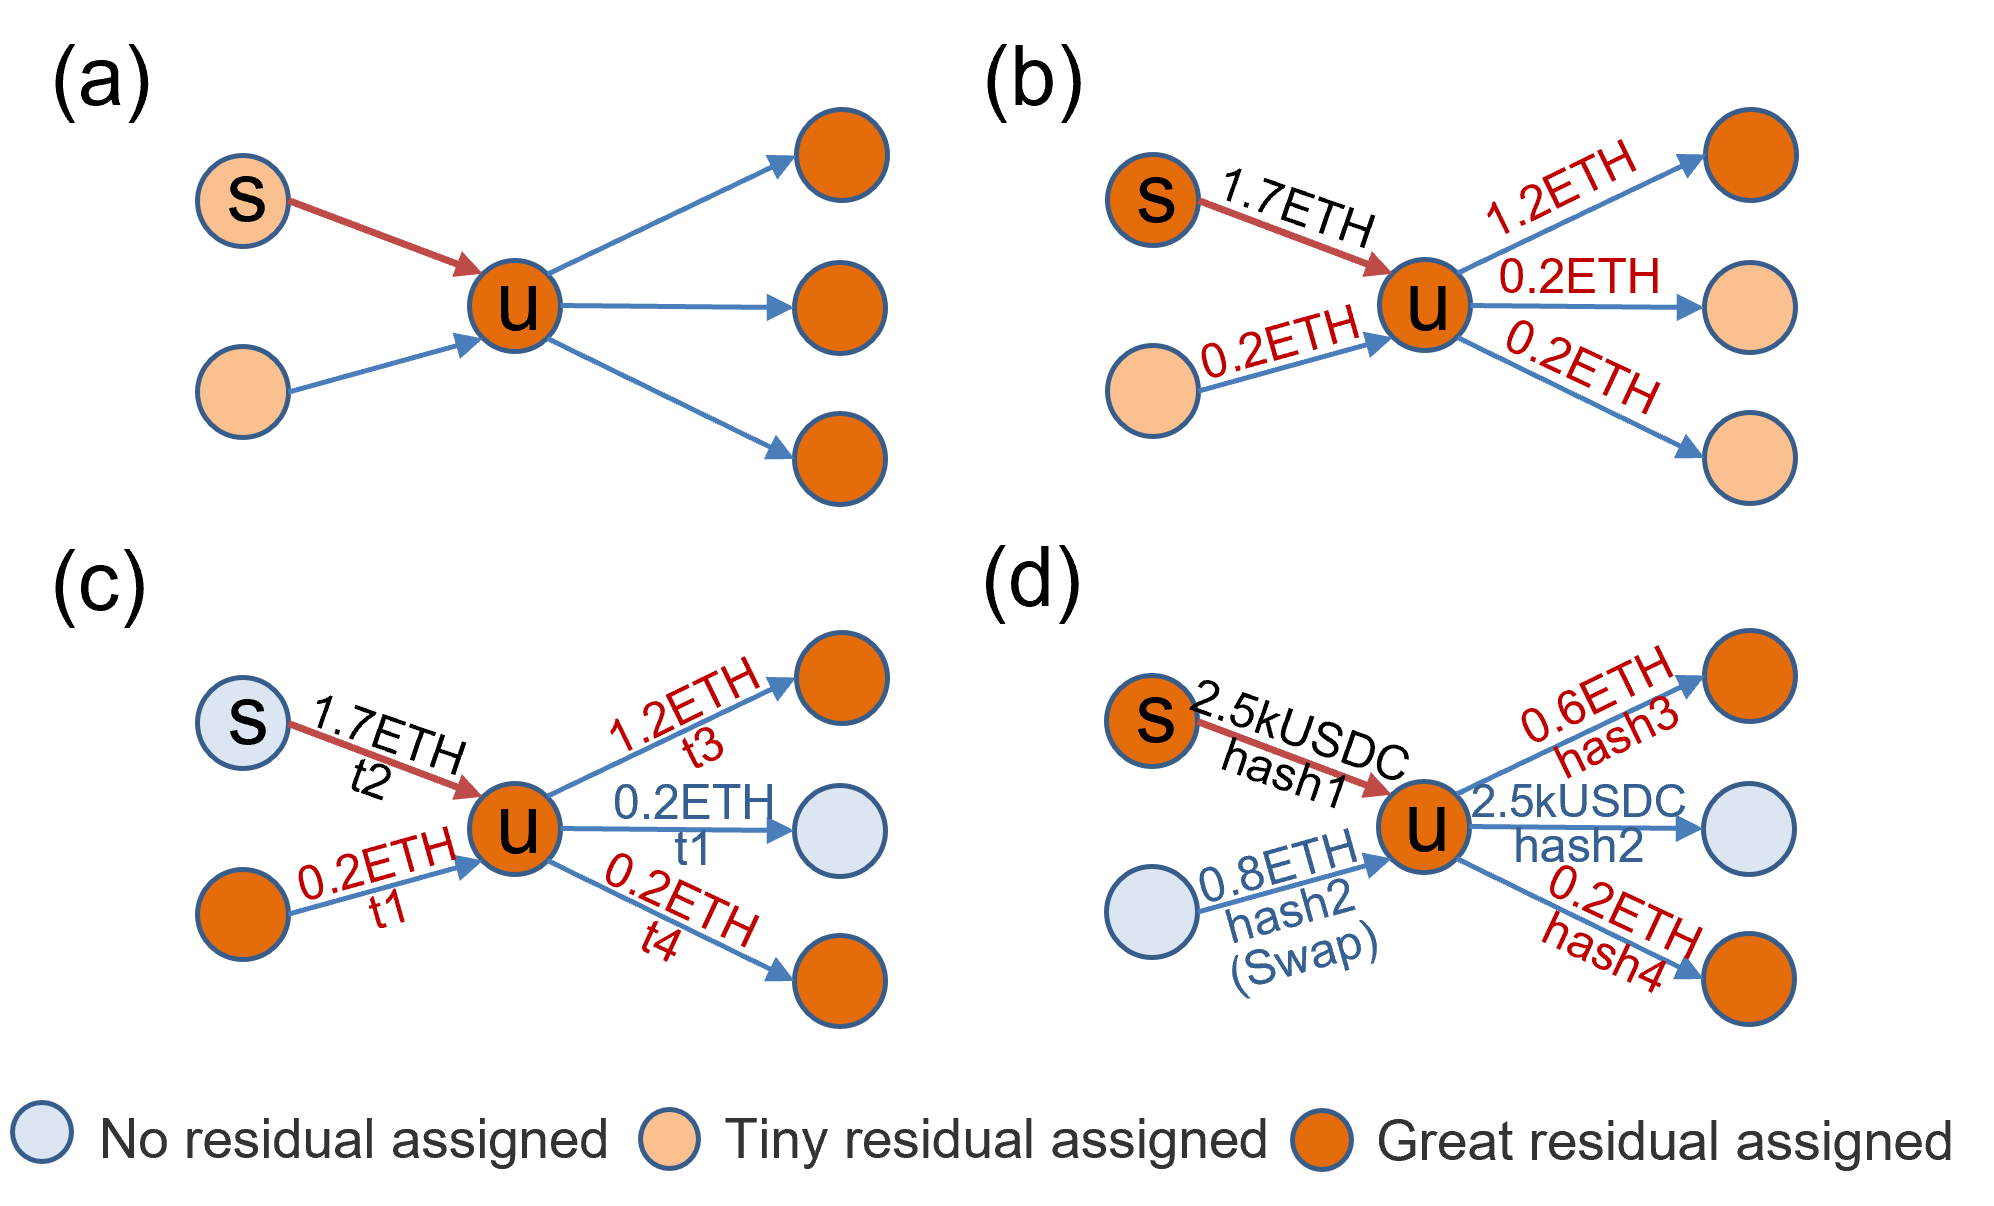
\includegraphics[width=0.9\linewidth]{figures/TTRstrategies.png}
    \caption{(a) Tracing tendency. 
    Different attention is assigned to the out-degree neighbors and in-degree neighbors.
    (b) Weighted pollution. The higher the edge weight, the closer the relationship. 
    (c) Temporal reasoning. Tracing money flow in chronological order, and $t1<t2<t3<t4$ in this example. 
    (d) Token redirection. Uncovering the token flows even though there exist complex DeFi actions in the Swap pattern.}
    \label{fig:TTR_strategies}
\end{figure}

% \begin{figure}[t]
%     \centering
%     \subfigure[Tracing tendency]{
%     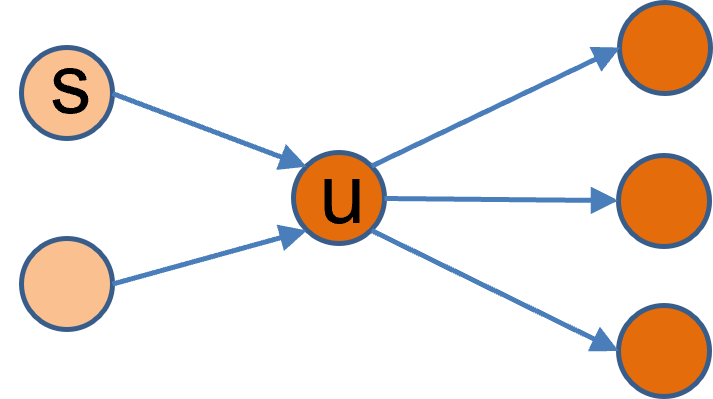
\includegraphics[width=0.35\linewidth]{figures/tracing_tendency.png}
%     \label{fig:tracing_tendency}
%     }
%     \subfigure[Weight pollution]{
%     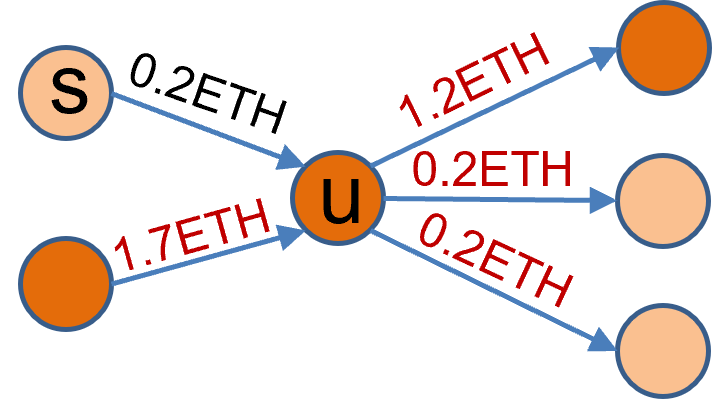
\includegraphics[width=0.35\linewidth]{figures/weight_pollution.png}
%     \label{fig:weight_pollution}
%     }
%     \subfigure[Temporal reasoning]{
%     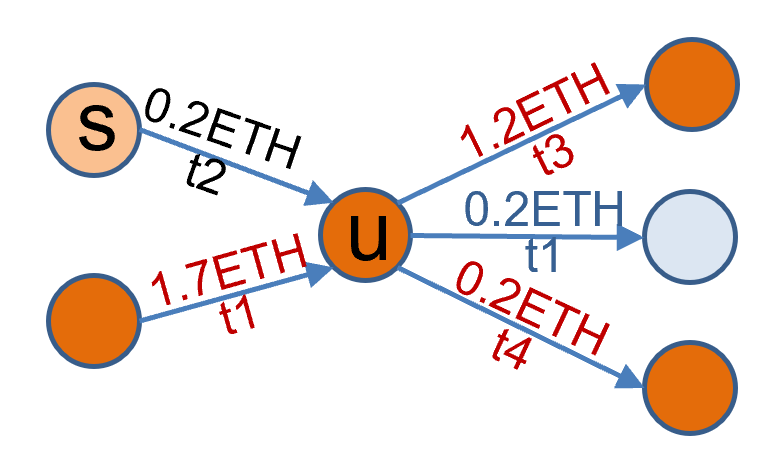
\includegraphics[width=0.35\linewidth]{figures/temporal_reasoning.png}
%     \label{fig:temporal_reasoning}
%     }
%     \subfigure[Token redirection]{
%     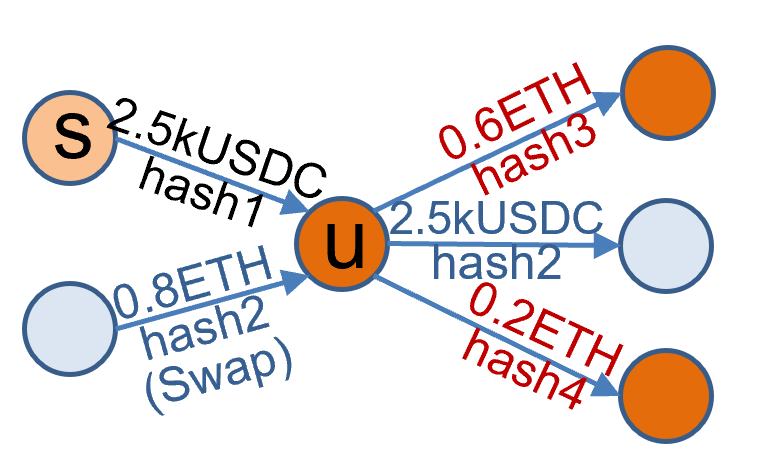
\includegraphics[width=0.35\linewidth]{figures/token_redirection.png}
%     \label{fig:token_redirection}
%     }
%     \caption{
%     (a) Tracing tendency. Different attention is assigned to the out-degree neighbors and in-degree neighbors.
%     (b) Weight pollution. The higher the edge weight, the closer the relationship. 
%     (c) Temporal reasoning. Tracing money flow in chronological order, and $t1<t2<t3<t4$ in this example. 
%     (d) Token redirection. Uncovering the token flow even though there exist complex transaction actions in the Swap pattern.
%     }
% \end{figure}

\textbf{Token redirection}.
% Besides native currency transfers, the transactions of account-based blockchain contain a large number of token transfers, while token redirection makes effort to reveal the real flow of interesting tokens.
This strategy makes the effort to uncover the flow of interesting tokens based on the transaction patterns of Xfer and Swap.
% In TRacer, the transaction patterns of Xfer and Swap are taken into consideration when it comes to tracing the token fund flow.
As Figure \ref{fig:TTR_strategies}(d) shows, the residual of node $u$ brought from the USDC token in an Xfer edge with hash1 should be pushed through the edges with hash3 and hash4, rather than the USDC outgoing edge with hash2. Since the edges with hash2 are in a Swap pattern and swapped the USDC token into ETH.
% As Figure \ref{fig:token_redirection} shows, the residual with USDC token received by the node $u$ in an Xfer edge with hash1 should have been pushed to the out-degree neighbor by the edge with USDC and hash2, but considering the edge with USDC and hash2 for redirection, the residual is pushed through the output edges with hash3 and hash4.
To achieve the redirection of token flows in complex transaction actions, we define a recursive function $\rho(\cdot,\cdot)$ which can find the initial state of a set of incoming edges before the Swap operations and the final state of a set of outgoing edges after the Swap operations within a node. For example, the initial state before Swap of the incoming edge with hash2 in Figure \ref{fig:TTR_strategies}(d) is the incoming edge with hash1, and the final state after Swap of the outgoing edge with hash2 is the outgoing edges with hash3 and hash4. More specifically, as shown in Algorithm \ref{alg:ttr_local_push} line 8-14, the residual of a specific token should be pushed through the redirected edges. Therefore, $\rho(\cdot,\cdot)$ satisfies the following recursive equation:
\begin{equation}\label{equation:token_redirect}
    \rho(\mathcal{E}, E(u))=\mathcal{E}_{xfer} \cup \rho(\bigcup\limits_{e \in \mathcal{E}_{swap}} redirect(e), E(u)),    
\end{equation}
where $\mathcal{E}$ is a set of edges for redirection, $\mathcal{E}_{xfer} \subset \mathcal{E}$ is a set of Xfer edges, $\mathcal{E}_{swap} \subset \mathcal{E}$ is a set of Swap edges, and $redirect(\cdot)$ selects the edges in the token types before/after Swap for incoming/outgoing edges $e \in \mathcal{E}_{swap}$ from edges $E(u)$ related to $u$.
% , which satisfies $f_{src}(e')=f_{src}(e)=u$ or $f_{tgt}(e')=f_{tgt}(e)=u$ for $\forall e' \in redirect(e)$.
% redirect selects the output/input edges from $E(u)$ with the swapped token symbol of the output/input edge $e \in \mathcal{E}_{swap}$.
Especially, $\rho(\emptyset, E(u)) = \emptyset$.

\subsubsection{\textit{Pop} and \textit{Expand}: Greedy Selection}
The \textit{Pop} operation selects a node from the subgraph for the next round expansion iteration, and the \textit{Expand} operation expands from a node by collecting all the related edges of this node.
% The \textit{Pop} operation selects a node with high priority from the subgraph in graph expansion, while \textit{Expand} collects all edges related to the selected node.
% In TRacer, the priority of the nodes is residual, where the node with a higher residual has a greater priority.
Note that the graph expansion in TRacer terminates when the residual of all nodes in the subgraph is below a threshold $\epsilon \in (0,1)$, i.e.,
\begin{equation}
    \max\limits_{u \in V}(\sum\limits_{t \in \Gamma}\sum\limits_{b \in B}r_s(u,t,b)) < \epsilon.
    \label{equ:end_cond}
\end{equation}
Thus we proposed the \textbf{greedy selection} for the \textit{Pop} operation to achieve the condition in Equation \ref{equ:end_cond}, i.e., the \textit{Pop} operation selects the node in the subgraph with the highest residual.
% Thus we proposed two types of node selection rules for the \textit{Pop} operation to achieve the condition in Equation \ref{equ:end_cond}, namely greedy selection, and group selection:
% \begin{itemize}
%     \item \textbf{Greedy selection}: Select one node in the subgraph with the highest residual.
%     \item \textbf{Group selection}: Select all nodes in the subgraph where the residual of every node is greater than $\epsilon$.
% \end{itemize}
% In our implementation, the greedy selection is chosen for \textit{Pop} operation enabled to reduce the pressure of data access in \textit{Expand}.

% \subsection{\textit{Extract}: Local Community Detection}
\subsection{Local Community Detection}
Referring to Figure~\ref{fig:TRacer}, the \textit{Extract} operation employs local community detection to construct a small-scale local community from the expanded graph. For a particular risky source node, the importance rank of the nodes within the local community is significantly higher than the external nodes, making it easy for further expert auditing.


The less conductance \cite{andersen2006local, andersen2007local} of the local community, the higher rank of the nodes in the local community than external nodes, in which the conductance is:
\begin{equation}
    \Phi(S)=\frac{\bm{p}_s(\partial(S))}{\bm{p}_s(S)},
\end{equation}
where $S$ denotes the nodes of the local community, the boundary $\partial(S)=\{ v| (u,v) \in E \land u \in S \land v \in \bar{S} \}$, $\bar{S}$ is the complement of $S$ and $\bm{p}_s(S)=\sum_{u \in S}\bm{p}_s(u)$ denotes the sum of rank over each node in the local community.
Given a specific threshold $\varphi > 0$ for conductance, the local community detection finds the local community satisfying:
\begin{equation}
    \Phi(S) < \varphi.
    \label{equ:local_comm_cond}
\end{equation}
With $S=\{s\}$ as the initialization, Algorithm \ref{alg:ttr_local_comm} describes how to find the local community satisfied the Equation \ref{equ:local_comm_cond}.
\begin{algorithm}[t]
    \caption{TTR-based Local Community Detection}
    \label{alg:ttr_local_comm}
    \begin{algorithmic}[1]
        \REQUIRE The source node $s$, the subgraph of graph expansion $G_s=(V_s, E_s)$, and the TTR score vector $\bm{p}_s$.
        \ENSURE The local community with nodes set $S$.
        \STATE $S = \{ s \}$
        \STATE $\bar{S} = V_s \setminus S$
        \WHILE{$\Phi(S) \geq \varphi$}
            \STATE $u =\mathop{\arg\max}_{v\in\bar{S}}\bm{p}_s(v)$
            % \STATE $u =$ the node with the highest rank in $\bar{S}$
            \STATE $S = S \cup \{ u \}$
            \STATE $\bar{S} = \bar{S} \setminus \{ u \}$
        \ENDWHILE
        \RETURN $G_s.subgraph(S)$
    \end{algorithmic}
\end{algorithm}
\subsection{Theoretical properties}
In this part, we discuss the theoretical properties of TRacer, and prove that our method is able to finish the transaction tracing task in large-scale transaction graphs with a constant time cost. Besides, we discuss the upper limit of the tracing depth in TRacer.

As the description in Proposition \ref{pot:cost}, the cost of TRacer is independent of the graph size, indicating that TRacer is able to trace on the large-scale transaction graph with a low cost.
\begin{proposition}
\label{pot:cost}
The iteration of graph expansion runs $O(\frac{1}{\epsilon \alpha})$ times, and the number of nodes with non-zero values in the output TTR score is at most $O(\frac{1}{\epsilon \alpha})$, which guarantees the cost of local community detection is $O(\frac{1}{\epsilon \alpha})$.
\end{proposition}
\begin{proof}
This follows from Andersen et al. \cite{andersen2006local}, Lemma 2.
\end{proof}

In addition, what depth can TRacer trace in a transaction graph from the source node is described in Proposition \ref{pot:max_depth}.
% where the higher order of the neighbor, the longer distance between the source node and this neighbor.
\begin{proposition}
\label{pot:max_depth}
An $n$-hop neighbor of the source node can be found in the graph obtained by graph expansion, in which $n$ satisfies:
\begin{equation}
    n \leq \frac{log(\epsilon)}{log(1-\alpha)} + 1.
\end{equation}
\end{proposition}
\begin{proof}
In order to maximize the rank of the neighbors far away from the source node, $\alpha$ needs to be as small as possible, and $\beta$ needs to be as close as possible to 0 or 1, which ensures that the residual can be pushed to a specific direction.
Let the sum of residual pushed from the source node $s$ to the $n$-hop neighbors be $r^{(n)}$.
Considering $\beta=1$ here, $r^{(n)}$ can be obtained by:
\begin{equation}
    \begin{cases}
        & r^{(1)}=(1-\alpha), \\
        & r^{(2)} \geq (1-\alpha)(r^{(1)}-k_1 \epsilon)=(1-\alpha)^2-(1-\alpha)k_1 \epsilon, \\
        & ...... \\
        & r^{(n)} \geq (1-\alpha)(r^{(n-1)}-k_{n-1} \epsilon) \\
        & \ \ \ \ \ \ \ \ =(1-\alpha)^n-\sum\limits_{i=1}^{n-1}(1-\alpha)^{n-i}k_{n-i} \epsilon, \\
    \end{cases}
\end{equation}
where $k_i$ represents the number of nodes with residual less than $\epsilon$ in the $i$-order neighbors of the source node.
Therefore, $r^{(n)}$ obtains the maximum value when:
\begin{equation}
    \sum\limits_{i=1}^{n-1}(1-\alpha)^{n-i}k_{n-i} \epsilon = 0,
\end{equation}
which means the residual of each $i$-order node is greater or equal than $\epsilon$. 
This situation exists when the source node is in a path-like graph, whose adjacency matrix $A$ satisfies $A(i,i+1)=1$ and other elements are $0$.
Considering the end condition of the local push procedure, the residual of $n$-hop neighbors is:
\begin{equation}
\begin{cases}
    & (1-\alpha)^n < \epsilon\\
    & (1-\alpha)^{n-1} \geq \epsilon \\
\end{cases}
    % r^{(n)}=(1-\alpha)^n \geq \epsilon
    \Rightarrow 
    \frac{log(\epsilon)}{log(1-\alpha)} < n \leq \frac{log(\epsilon)}{log(1-\alpha)} + 1.
    % n \leq \frac{log(\epsilon)}{log(1-\alpha)}.
\end{equation}
\end{proof}
% ------------ 旧版内容 ------------
% \subsection{Push-Pop Model}
% In this paper, we propose a general framework called Push-Pop model for transaction tracking on blockchain trading systems. 
% As shown in Figure \ref{fig:push_pop_model}, the Push-Pop model starts from the source node $s$ with a specific transaction tracking strategy $T$, builds a witnessed network iteratively, and finds a subgraph from the witnessed network as the local tracking network of the source node finally.
% Here we aim to find a local tracking network containing as many target nodes as possible.
% The witnessed network of a source node under a transaction tracking strategy $T$ is defined as $G_s^T=(V_s^T,E_s^T,PR_s^T)$, where $V_s^T$ and $E_s^T$ denote the nodes and edges of $G_s^T$ respectively while $PR_s^T$ is a vector denoting the priority of all nodes in $G_s^T$.

% To build $G_s^T$ for source node $s$, the steps of Push-Pop model are defined as follows:
% \begin{enumerate}
%     \item \textit{initialize}: Let $V_s^{T}=\{ s \}$, $E_s^{T}=\emptyset$, and $PR_s^T(s)=1$.
%     \item \textit{pop}: Output the node $v$ with the highest priority from the node set $V_s^{T}$.
%     \item \textit{expand}: Query the edges $E(v)$ related to $v$ and the neighbor nodes $N(v)$ of $v$.
%     \item \textit{push}: Update the witnessed network $G_s^T$ in which $E_s^{T}=E_s^{T} \cup E(v)$, $V_s^{T}=V_s^{T} \cup N(v)$, and employ the transaction tracking strategy $T$ to rank the priority of nodes in $V_s^T$ for updating $PR_s^{T}$. If the end condition of $T$ is not satisfies, go to step 2.
%     \item \textit{extract}: Output a subgraph of the witnessed network $G_s^T$ as the local tracking network $G_s$.
% \end{enumerate}

% % Therefore, the Push-Pop model is defined as Algorithm \ref{alg:push_pop}.
% Obviously, the effectiveness of Push-Pop model depends on the transaction tracking strategy, and how to design an effective strategy will be discussed in the next part.
% % \begin{algorithm}[htb]
% %     \caption{Push-Pop Model}
% %     \label{alg:push_pop}
% %     \begin{algorithmic}[1]
% %         \REQUIRE The transaction network $G$, the source node $s$, transaction tracking strategy $T$
% %         \ENSURE The local tracking network captured by $T$
% %         \STATE $T.V.init(s)$
% %         \WHILE{$T.V.hasNext()$}
% %             \STATE $u = T.V.pop()$
% %             \STATE $E(u) = T.expand(u)$
% %             \STATE $T.V.push(E(u))$
% %         \ENDWHILE
% %         \RETURN $T.extract(G_T)$
% %     \end{algorithmic}
% % \end{algorithm}

% \subsection{Transaction Tracking Rank Algorithm}
% The TTR algorithm improves the local push procedure of APPR to enable that nodes related to the source node in a given transaction network $G=(V,E)$ can have a higher estimate of $\bm{p}_s$.
% According to the attributes of transaction network, we design three local push strategies in the TTR algorithm.

% % \begin{figure*}[htb]
% %     \centering
% %     \subfigure[tracking tendency]{
% %         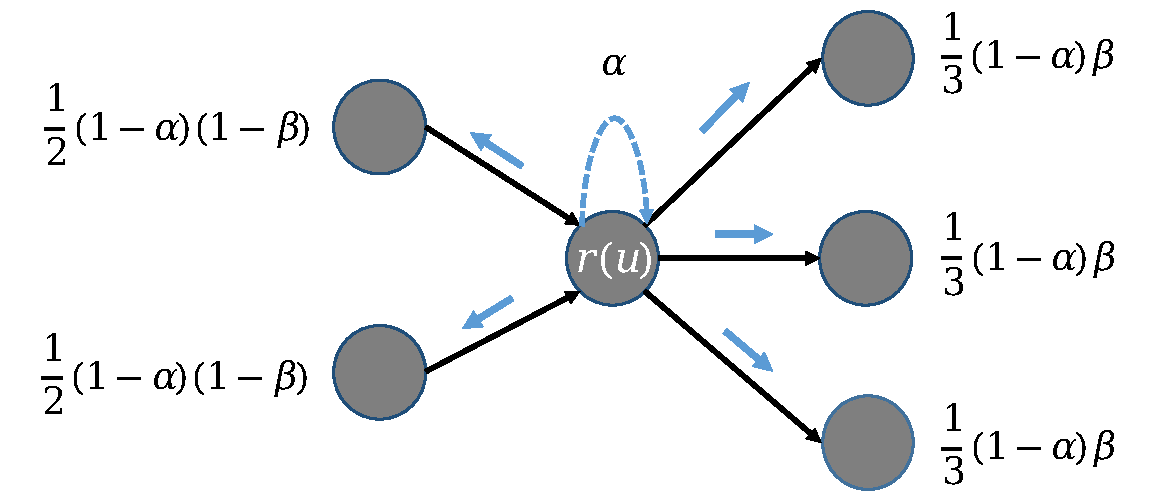
\includegraphics[width=0.3\linewidth]{figures/local_push_ttr_base.pdf}
% %         \label{fig:local_push_ttr_base}
% %     }
% %     \subfigure[weight pollution]{
% %         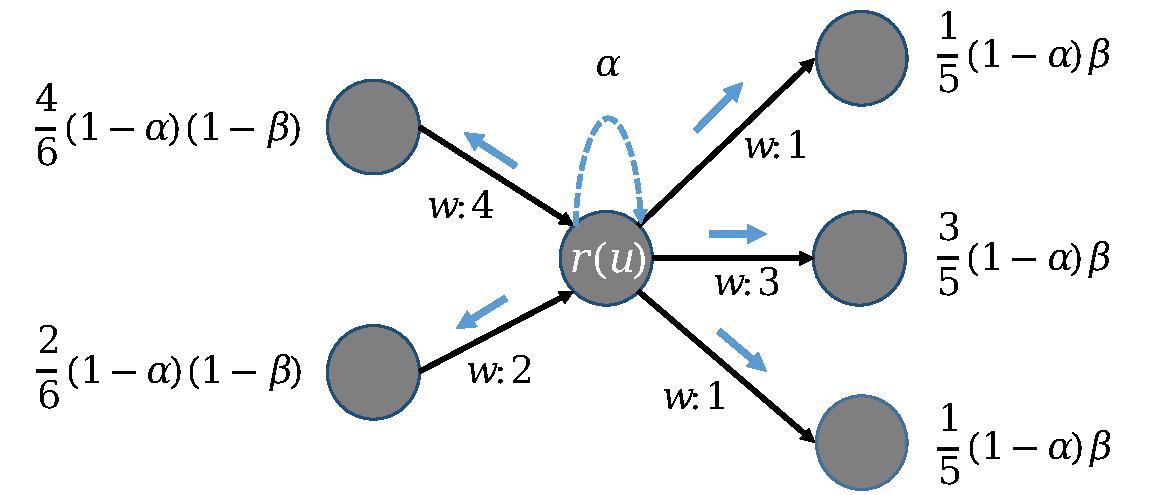
\includegraphics[width=0.3\linewidth]{figures/local_push_ttr_weight.pdf}
% %         \label{fig:local_push_ttr_weight}
% %     }
% %     \subfigure[temporal reasoning]{
% %         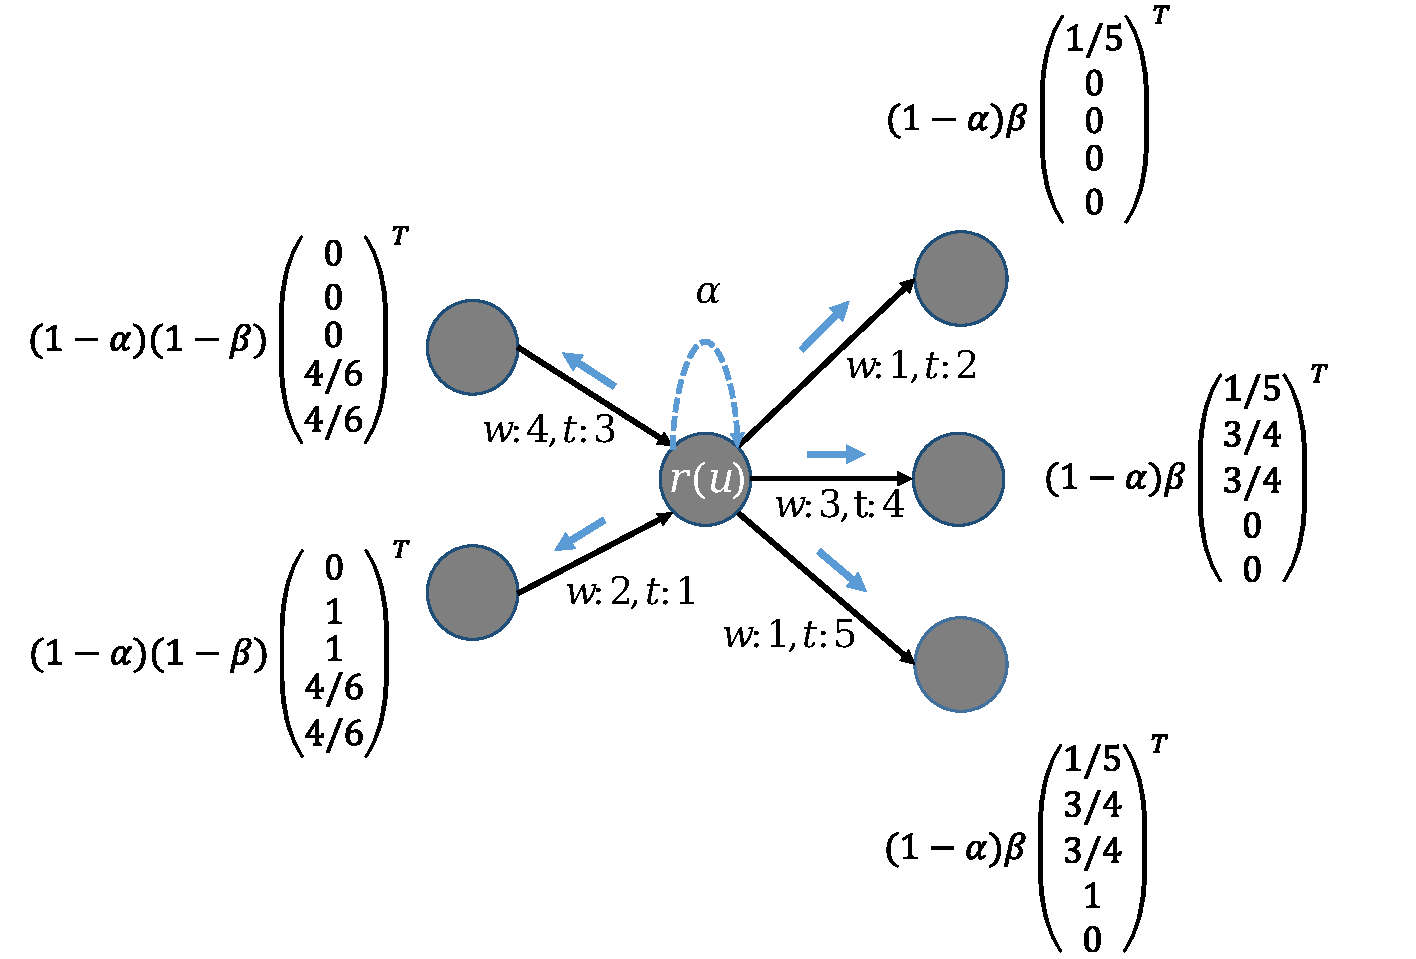
\includegraphics[width=0.3\linewidth]{figures/local_push_ttr_time.pdf}
% %         \label{fig:local_push_ttr_time}
% %     }
% %     \caption{TTR.}
% % \end{figure*}

% % 介绍三种递进的push策略
% \subsubsection{Tracking tendency}
% Since a transaction relationship between addresses is directed, during the transaction tracking process, the attention to in-degree neighbors and out-degree neighbors may be different. 
% For example, tracking for the target of the fund flows oriented from a particular needs to pay more attention to its out-degree neighbors, while searching for the source of money needs to pay more attention to the in-degree neighbors.
% Therefore, considering the transaction network $G$ as a directed graph and giving a tracking tendency coefficient $\beta \in [0,1]$, the out-degree neighbors in a transaction relationship can get a higher estimate of $\bm{p}_s$ when $\beta > 0.5$, and the in-degree neighbors in a transaction relationship can get a higher estimate of $\bm{p}_s$ when $\beta < 0.5$.
% % The local push procedure can push the residual to self, out-degree neighbors, and in-degree neighbors with different ratios.
% In this way, Equation \ref{equ:ppr} can be re-written as:
% \begin{equation}
%     \bm{p}_s = \alpha \bm{e}_s + (1-\alpha) \bm{p}_s M_{\beta}.
%     \label{equ:ttr_base}
% \end{equation}
% The transition matrix of Equation \ref{equ:ttr_base} is:
% \begin{equation}
%     M_{\beta} = \beta D_{out}^{-1}A + (1-\beta)D_{in}^{-1}A^T,
% \end{equation}
% where $A$ is the adjacency matrix of $G$, $D_{out}$ is an out-degree matrix of $G$, and $D_{in}$ is an in-degree matrix of $G$.

% In this way, the local push procedure of node $u$ pushes the residual to itself, out-degree neighbors, and in-degree neighbors. 
% And each in-degree neighbor and each out-degree neighbor receive an equal proportion depending on the in-degree and out-degree, respectively.
% Therefore, Equations \ref{equ:local_push_appr} can be re-written as:
% \begin{equation}
%     \begin{cases}
%         & \bm{p}_s(u)=\bm{p}_s(u)+\alpha \bm{r}_s(u) \\ 
%         & \bm{r}_s(v_{out})=\bm{r}_s(v_{out})+\theta_{\beta}(u,v_{out}) \bm{r}_s(u) \\ 
%         & \bm{r}_s(v_{in})=\bm{r}_s(v_{in})+\theta_{\beta}(u,v_{in}) \bm{r}_s(u)
%     \end{cases},
%     \label{equ:local_push_ttr_base}
% \end{equation}
% where $v_{out} \in N_G^{out}(u)$ and $v_{in} \in N_G^{in}(u)$ denote out-degree neighbor and in-degree neighbor of $u$ respectively, and the push factors are defined as follows:
% \begin{equation}
%     \theta_{\beta}(u,v_{out})=\frac{(1-\alpha)\beta}{d_{out}(u)},
% \end{equation}
% \begin{equation}
%     \theta_{\beta}(u,v_{in})=\frac{(1-\alpha)(1-\beta)}{d_{in}(u)},
% \end{equation}
% in which $d_{out}(u)$ and $d_{in}(u)$ denote out-degree and in-degree of $u$ respectively.
% % \begin{figure}[htb]
% %     \centering
% %     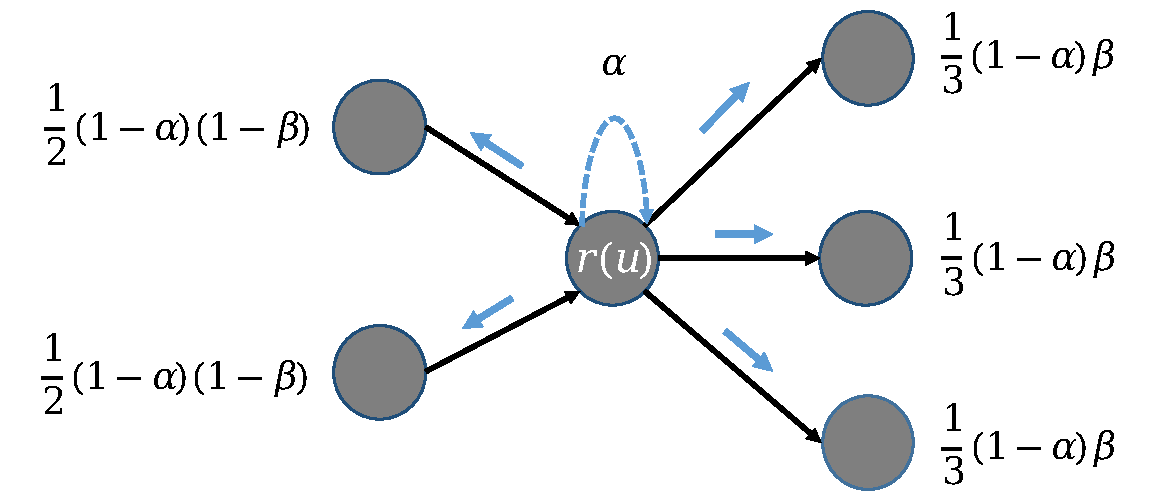
\includegraphics[width=\linewidth]{figures/local_push_ttr_base.pdf}
% %     \caption{Local push procedure with tracking tendency}
% %     \label{fig:local_push_ttr_base}
% % \end{figure}
% And if a node $u$ has no out-degree neighbors or in-degree neighbors, the residual can be pushed to itself.
% % \begin{equation}
% %     r(u)=r(u)+(1-\alpha)\beta r(u),
% % \end{equation}
% % \begin{equation}
% %     r(u)=r(u)+(1-\alpha)(1-\beta) r(u).
% % \end{equation}


% \subsubsection{Weight pollution}
% Traditional APPR pushes the residual of a node to the neighbors by considering an equal weight during a local push iteration. However, in a transaction relationship, the transaction strength is usually weighted by the transaction amount. For each node in the network, a neighbor who has transaction relationships with a larger amount of money is considered to be more relevant to the node. 
% % For example, tracking the fund flow of a node $u$ needs to pay more attention to the neighbors having a large amount of transactions related to $u$.
% % In the procedure of transaction tracking, attention to the nodes whether related to the source node on the amount is needed.
% % For example, the amount received by some nodes is similar to the amount output by the source node, these nodes may be related to the source node.
% Therefore, by considering the transaction network $G$ as a weighted directed graph with the transaction amount information as the weight, Equation \ref{equ:ttr_base} can be re-written as:
% %the nodes get a higher estimate of $\bm{p}_s$ when these nodes have a significant association with the source node on the perspective of edge weight.
% \begin{equation}
%     \bm{p}_s = \alpha \bm{e}_s + (1-\alpha) \bm{p}_s M_w.
%     \label{equ:ttr_weight}
% \end{equation}
% The transition matrix of Equation \ref{equ:ttr_weight} is:
% \begin{equation}
%     % M_w = \beta {D_{out}^w}^{-1}W + (1-\beta){D_{in}^w}^{-1}W^T,
%     M_w = \beta \tilde{D}_{out}^{-1}W + (1-\beta)\tilde{D}_{in}^{-1}W^T,
% \end{equation}
% where $W$ is the weighted adjacency matrix of $G$, $\tilde{D}_{out}$ is the weighted out-degree matrix of $G$, $\tilde{D}_{in}$ is the weighted in-degree matrix of $G$. 
% The diagonal elements of $\tilde{D}_{out}$ and $\tilde{D}_{in}$ are defined as follows:
% \begin{equation}
%     \tilde{D}_{out}(i,i)=||W(i,)||,
% \end{equation}
% \begin{equation}
%     \tilde{D}_{in}(i,i)=||W^T(i,)||, i\leq|V|
% \end{equation}
% where $W(i,)$ and $W^T(i,)$ denote the $i$-th row in $W$ and $W^T$ respectively. All off-diagonal elements in $\tilde{D}_{out}$ and $\tilde{D}_{in}$ equal to 0.

% In this way, the local push procedure of node $u$ pushes residual to itself, the out-degree neighbors and the in-degree neighbors with different ratios determined by edge weight. And Equations \ref{equ:local_push_ttr_base} can be re-written as:
% % \begin{equation}
% %     \begin{cases}
% %       & p(u)=p(u)+\alpha r(u), \\ 
% %       & r(\hat{v})=r(\hat{v})+(1-\alpha)\beta \frac{W(u,\hat{v})}{W(u,)} r(u), \\ 
% %       & r(\tilde{v})=r(\tilde{v})+(1-\alpha)(1-\beta) \frac{W(\tilde{v},u)}{W(,u)} r(u),
% %     \end{cases}
% % \end{equation}
% \begin{equation}
%     \begin{cases}
%       & \bm{p}_s(u)=\bm{p}_s(u)+\alpha \bm{r}_s(u) \\ 
%       & \bm{r}_s(v_{out})=\bm{r}_s(v_{out})+\theta_w(u,v_{out}) \bm{r}_s(u) \\ 
%       & \bm{r}_s(v_{in})=\bm{r}_s(v_{in})+\theta_w(u,v_{in}) \bm{r}_s(u)
%     \end{cases},
%     \label{equ:local_push_weight}
% \end{equation}
% where the push factors are defined as follows:
% \begin{equation}
%     \theta_w(u,v_{out})=(1-\alpha)\beta\frac{w(u,v_{out})}{\tilde{d}_{out}(u)},
% \end{equation}
% \begin{equation}
%     \theta_w(u,v_{in})=(1-\alpha)(1-\beta)\frac{w(v_{in},u)}{\tilde{d}_{in}(u)},
% \end{equation}
% in which $w(u,v)$ for $\forall{u,v \in V}$ denotes the transaction amount from $u$ to $v$, and $\tilde{d}_{out}(u)$ and $\tilde{d}_{in}(u)$ denote the weighted out-degree and weighted in-degree of $u$ respectively.
% % \begin{figure}[htb]
% %     \centering
% %     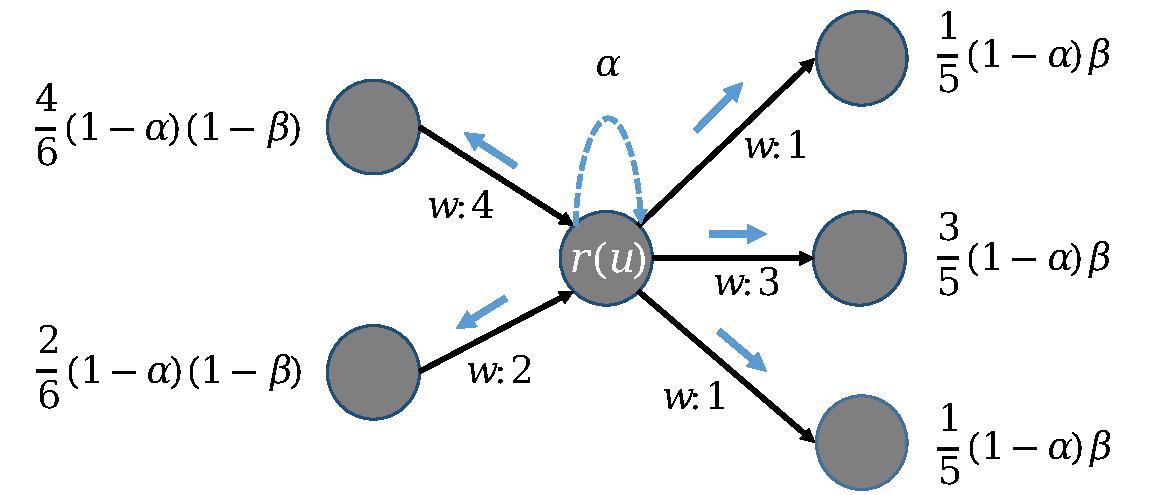
\includegraphics[width=\linewidth]{figures/local_push_ttr_weight.pdf}
% %     \caption{Local push procedure with weight pollution}
% %     \label{fig:local_push_ttr_weight}
% % \end{figure}

% \subsubsection{Temporal reasoning} Blockchain transactions are recorded in blocks chronologically, and each block contains a specific timestamp. Since the fund flow transferring process is dynamic, the transaction time information can be taken into consideration in the local push procedure.
% % Since a transaction relationship is temporal, during the transaction tracking process, the attention to the neighbors may be different.
% In the scenario of blockchain transaction tracking, tracking for the target of a fund flow usually follows the paths with increasing timestamps, while tracking back to the source of a fund flow follows the paths with decreasing timestamps.
% % In the procedure of transaction tracking, starting from the source node, the nodes in the increasing timestamp fund flow or decreasing timestamp fund flow get higher importance.
% % Therefore, considering the transaction network $G$ as a temporal weighted directed graph in which $G^{(t)}$ denotes the weighted directed graph at the $t$-th timestamp, for all timestamp indices $\{1,2, ...,t, ..., t_{\rm max} \}$
% % in $G$, Equation \ref{equ:ttr_weight} can be re-written as:
% Therefore, considering the transaction network $G$ as a temporal weighted directed graph in which $G^{(t)}$ denotes the weighted directed graph at timestamp $t$, for all timestamp $\{ t_1,...,t_k,...,t_n \}$ in $G$, Equation \ref{equ:ttr_weight} can be re-written as:
% \begin{equation}
%     \bm{p}_s^{(t)} = \alpha \bm{e}_s^{(t)} + (1-\alpha) p_s^{(t)} M_w^{(t)},
%     \label{equ:ttr}
% \end{equation}
% where $\bm{p}_s^{(t)}$ denotes the estimate of $\bm{p}_s$ at timestamp $t$, $M_w^{(t)}$ denotes the transition matrix at timestamp $t$, and $\bm{e}_s^{(t)}$ denotes the indicator vector at timestamp $t$ in which $\bm{e}_s^{(t_1)}=\bm{e_s}$ and $\bm{e}_s^{(t_k)} = \bm{p}_s^{(t_{k-1})}$.
% % where $P_s$ is a $t_{max} \times |V|$ matrix in which each row $P_s(t,)$ denotes the importance of all nodes to the source node at $t$-th timestamp.
% % element $\bm{P}_s^{(t)}(u)$ is able to describe the importance of node $u$ to the source node at time $t$
% In this case, $\bm{p}_s$ is redefined as follow:
% \begin{equation}
%     % \bm{p}_s=\sum\limits_{t=1}^{t_{\rm max}}{P_s(t,)}.
%     \bm{p}_s=\frac{1}{n}\sum\limits_{t{'}=t_1}^{t_n}{\bm{p}_s^{(t{'})}}.
% \end{equation}
% % , and the estimate of $p$ can be re-written as $p=\sum_t{p_{\infty}^{(t)}}$.
% The transition matrix of Equation \ref{equ:ttr} is:
% \begin{equation}
%     % M_{t} = \beta \hat{D}_{out}^{-1}W_{t} + (1-\beta)\hat{D}_{in}^{-1}W_{t}^T,
%     % M_{T} = \beta \hat{D}_{out}^{-1}\mathcal{W} + (1-\beta)\hat{D}_{in}^{-1}\mathcal{W}^T,
%     M_{w}^{(t)} = \beta \hat{D}_{out}^{{(t)}^{-1}} W^{(t)} + (1-\beta)\hat{D}_{in}^{{(t)}^{-1}} W^{{(t)}^T},
% \end{equation}
% where $W^{(t)}$ is a weighted adjacency matrix at timestamp $t$, $\hat{D}_{out}^{(t)}$ and $\hat{D}_{in}^{(t)}$ denote the cumulative weighted out-degree matrix and the cumulative weighted in-degree matrix at timestamp $t$ respectively.
% % where $\mathcal{W}$ is a $t_{\rm max} \times |V| \times |V|$ tensor in which $\mathcal{W}(t,)$ denotes the weighted adjacency matrix at the $t$-th timestamp, $\hat{D}_{out}$ and $\hat{D}_{in}$ record the weighted out-degree matrix and the weighted in-degree matrix in each timestamp respectively with the same dimension as $\mathcal{W}$. 
% % $\hat{D}_{out}$ is a temporal weighted out-degree matrix of $G$, 
% % $\hat{D}_{in}$ is a temporal weighted in-degree matrix of $G$, 
% % and $\hat{D}_{out}$ and $\hat{D}_{in}$ have the same dimensions as $W_{t}$.
% The nonzero elements of $\hat{D}_{out}$ and $\hat{D}_{in}$ are defined as follows:
% \begin{equation}
%     % \hat{D}_{out}(t,i,i)=\sum\limits_{t{'}>t}||\mathcal{W}(t',i,)||,
%     \hat{D}_{out}^{(t)}(i,i)=\sum\limits_{t{'}\leq t}||W^{(t{'})}(i,)||,
% \end{equation}
% \begin{equation}
% %   \hat{D}_{in}(t,i,i)=\sum\limits_{t{'}<t}||\mathcal{W}^T(t',i,)||, t\leq t_{\rm max}, i\leq|V|,
%     \hat{D}_{in}^{(t)}(i,i)=\sum\limits_{t{'}\geq t}||W^{(t{'})}(,i)||, t_1 \leq t\leq t_{n}, i\leq|V|,
% \end{equation}
% in which $W^{(t{'})}(i,)$ and $W^{(t{'})}(,i)$ denote the $i$-th row and the $i$-th column in the weighted adjacency matrix at timestamp $t{'}$ respectively.
% % Especially, $\hat{D}_{out}=\tilde{D}_{out}$ and $\hat{D}_{in}=\tilde{D}_{in}$ at timestamp $t_1$.
% % in which $\mathcal{W}(t,i,)$ denotes the row $i$ in the weighted adjacency matrix at the $t$-th timestamp respectively.
% % \begin{equation}
% %     \hat{D}_{t}(i,j,j)=\hat{d}_{t}^{(t_i)}(v_j)=\sum\limits_{t{'}>t}||W_{t}(i,j)||,
% % \end{equation}
% % \begin{equation}
% %   \tilde{D}_{t}(i,j,j)=\tilde{d}_{t}^{(t_i)}(v_j)=\sum\limits_{t{'}<t}||W_{t}^T(i,j)||,
% % \end{equation}
% % in which $W_{t}(i,j)$ and $W_{t}^T(i,j)$ denote the rows $j$ in $W_{t}$ and $W_{t}^T$ at timestamp $t_i$ respectively.

% In this way, the local push procedure of node $u$ pushes the residual to itself, out-degree neighbors, and in-degree neighbors with different ratios determined by the transaction amount and time.
% Equations \ref{equ:local_push_weight} can be re-written as:
% % \begin{equation}
% %     \begin{cases}
% %       & \bm{p}_s(u)=\bm{p}_s(u)+\alpha \bm{e} \cdot R_s(u), \\ 
% %       & R_s(\hat{v})=R_s(\hat{v})+\theta_{t}(u,\hat{v}) \odot R_s(u), \\ 
% %       & R_s(\tilde{v})=R_s(\tilde{v})+\theta_{t}(u,\tilde{v}) \odot R_s(u),
% %     \end{cases}
% % \end{equation}
% \begin{equation}
%     \begin{cases}
%       & \bm{p}_s(u)=\bm{p}_s(u)+\alpha \bm{e} \cdot R_s(u) \\ 
%       & R_s(v_{out})=R_s(v_{out})+\theta_{t}(u,v_{out}) \odot R_s(u) \\ 
%       & R_s(v_{in})=R_s(v_{in})+\theta_{t}(u,v_{in}) \odot R_s(u)
%     \end{cases},
% \end{equation}
% where $R_s$ denotes a $n \times |V|$ matrix in which $R_s(v_i)=R_s(,i)$ denotes the residual of a node $v_i$ at each timestamp, $\odot$ denotes the element-wise product, and the push factors are defined as follows:
% % where $R_s$ denotes a $n \times |V|$ matrix in which $R_s(v_i)=R_s(,i)$ denotes the residual of a node $v_i$ at each timestamp, $\odot$ denotes the element-wise product, and the push factors are defined as follows:
% % \begin{equation}
% %     \theta_{t}(u,\hat{v})=(1-\alpha)\beta w_{t}(u,\hat{v}) \oslash \hat{d}_{t}(u),
% % \end{equation}
% % \begin{equation}
% %     \theta_{t}(u,\tilde{v})=(1-\alpha)(1-\beta) w_{t}(\tilde{v},u) \oslash \tilde{d}_{t}(u),
% % \end{equation}
% \begin{equation}
%     \theta_{t}(u,v_{out})=(1-\alpha)\beta w_{t}(u,v_{out}) \oslash \hat{d}_{out}(u),
% \end{equation}
% \begin{equation}
%     \theta_{t}(u,v_{in})=(1-\alpha)(1-\beta) w_{t}(v_{in},u) \oslash \hat{d}_{in}(u),
% \end{equation}
% in which $w_{t}(u,v)$ for $\forall{u,v \in V}$ is a vector denoting the transaction amount from $u$ to $v$ at each timestamp, $\hat{d}_{out}(u)$ and $\hat{d}_{in}(u)$ denote the temporal weight out-degree and in-degree at each timestamp respectively, and $\oslash$ denotes the element-wise division.

% Based on the above local push strategies, we propose the TTR algorithm.
% Giving a transactions network $G=(V,E)$, TTR tracking for the target starting from the source node $s$.
% Initializing $R_s$ with edges related to $s$, TTR calls the local push procedure to push the residual for a node itself, the out-degree neighbors, and the out-degree neighbors by ``selfPush", ``forwardPush" and ``backwardPush"  procedure respectively, until the residual of each node is within the minimum error $\epsilon$.
% % initializes the estimate $p=\vec{0}$ and the temporal residual $r_{\infty}$, and then 
% % call the local push procedure to push the residual for self, out-degree neighbors and out-degree neighbors by ``selfPush", ``forwardPush" and ``backwardPush"  procedure respectively, until the residual of each node within the minimum error $\epsilon$.
% Algorithm \ref{alg:ttr} describes the framework of the TTR algorithm, Algorithm \ref{alg:self_push}, Algorithm \ref{alg:forward_push} and Algorithm \ref{alg:backward_push} describe the ``selfPush", ``forwardPush" and ``backwardPush" procedure in detail respectively.
% \begin{algorithm}[t]
%     \caption{Transaction Tracking Rank}
%     \label{alg:ttr}
%     \begin{algorithmic}[1]
%         \REQUIRE Source node $s$, transactions network $G=(V,E)$ with timestamp range $\{t_1,t_2,...,t_n\}$, teleport constant $\alpha$, minimum error $\epsilon$, and tracking tendency coefficient $\beta$.
%         \ENSURE the estimate of $\bm{p}_s$
%         \STATE $\bm{p}_s(s)=\alpha$
%         \STATE $R_{s}(t,v)=(1-\alpha)\beta w/\tilde{d}_{out}(s)$ for $\forall{(s,v,w,t)} \in E_{out}(s)$
%         \STATE $R_{s}(t,v)=(1-\alpha)(1-\beta) w/\tilde{d}_{in}(s)$ for $\forall{(v,s,w,t)} \in E_{in}(s)$
%         \IF{$E_{out}(s)=\emptyset$}
%             \STATE $R_s(t_1,s)=(1-\alpha)\beta$
%         \ENDIF
%         \IF{$E_{in}(s)=\emptyset$}
%             \STATE $R_s(t_n,s)=(1-\alpha)(1-\beta)$
%         \ENDIF
%         \WHILE{$||R_s(u)|| \geq \epsilon, u \in V$}
%             \STATE Let $R_s^{\prime}=R_s$, and $R_{s}(u)=\vec{0}$.
%             \STATE Apply $R_s^{\prime}$ to update $\bm{p}_s$ and $R_s$ through selfPush, forwardPush and backwardPush.  
%         \ENDWHILE
%         \RETURN $\bm{p_s}$
%     \end{algorithmic}
% \end{algorithm}

% \begin{algorithm}[t]
%     \caption{selfPush}
%     \label{alg:self_push}
%     \begin{algorithmic}[1]
%         \REQUIRE Node $u$, temporal residual $R_s^{\prime}$, estimate $\bm{p}_s$, and teleport constant $\alpha$.
%         \FOR{$t \in [t_1, t_n]$}
%             \STATE $\bm{p}_s(u)+=\alpha R_s^{\prime}(t,u)$
%         \ENDFOR
%     \end{algorithmic}
% \end{algorithm}

% \begin{algorithm}[t]
%     \caption{forwardPush}
%     \label{alg:forward_push}
%     \begin{algorithmic}[1]
%         \REQUIRE Node $u$, out-edges $E_{out}(u)$, temporal residual $R_s^{\prime}$ and $R_s$, teleport constant $\alpha$, and tracking tendency coefficient $\beta$.
%         \FOR{$\forall{e:(u,v,w,t)} \in E_{out}(u)$}
%             \STATE $\Delta = 0$
%             \FOR{$\tau \in [t_1,t]$}
%                 \STATE $\Delta += w R_s^{\prime}(\tau,u) / \hat{d}_{out}^{(\tau)}(u)$
%                 % \STATE $\Delta += w{\rho}_{\infty}^{(\tau)}(u) / \hat{d}_{\infty}^{(\tau)}(u)$
%             \ENDFOR
%             % \STATE $r^{(t)}_{\infty}(\hat{v})+=(1-\alpha) \beta \Delta$
%             \STATE $R_s(t,v) += (1-\alpha)\beta \Delta$
%         \ENDFOR
%         \STATE Calculate $max(t)$ from all $t$ in $E_{out}(u)$.
%         \FOR{$\tau \in [max_t, t_n]$}
%             % \STATE $r_{\infty}^{(\tau)}(u)+=(1-\alpha)\beta {\rho}_{\infty}^{(\tau)}(u)$
%             \STATE $R_s(\tau,u) += (1-\alpha)\beta R_s^{\prime}(\tau,u)$
%         \ENDFOR
%     \end{algorithmic}
% \end{algorithm}

% \begin{algorithm}[t]
%     \caption{backwardPush}
%     \label{alg:backward_push}
%     \begin{algorithmic}[1]
%         \REQUIRE Node $u$, in-edges $E_{in}(u)$, temporal residual $R_s^{\prime}$ and $R_s$, teleport constant $\alpha$, and tracking tendency coefficient $\beta$.
%         \FOR{$\forall e:(v,u,w,t) \in E_{in}(u)$}
%             \STATE $\Delta = 0$
%             \FOR{$\tau \in [t, t_n]$}
%                 % \STATE $\Delta += w{\rho}_{\infty}^{(\tau)}(u) / \tilde{d}_{\infty}^{(\tau)}(u)$
%                 \STATE $\Delta += w R_s^{\prime}(\tau, u) / \hat{d}_{in}^{(\tau)}(u)$
%             \ENDFOR
%             % \STATE $r_{\infty}^{(t)}(\tilde{v}) += (1-\alpha)(1-\beta)\Delta$
%             \STATE $R_s(t,v) += (1-\alpha)(1-\beta)\Delta$
%         \ENDFOR
%         \STATE Calculate $min(t)$ from all $t$ in $E_{in}(u)$.
%         \FOR{$\tau \in [t_1, min(t)]$}
%             % \STATE $r_{\infty}^{(\tau)}(u)+=(1-\alpha)(1-\beta) {\rho}_{\infty}^{(\tau)}(u)$
%             \STATE $R_s(\tau,u)+=(1-\alpha)(1-\beta) R_s^{\prime}(\tau,u)$
%         \ENDFOR
%     \end{algorithmic}
% \end{algorithm}

% % \begin{algorithm}[htb]
% %     \caption{forwardPush}
% %     \label{alg:forward_push}
% %     \begin{algorithmic}[1]
% %         \REQUIRE node $u$, out-edges set of node $E(u,)$, residual vector $r$, tracking tendency coefficient $\alpha$ and $\beta$.
% %         \STATE // sort $E(u,)$ and $r(u)$ by timestamp increasingly
% %         \STATE $E(u,)=sort(E(u,))$ 
% %         \STATE $r(u)=sort(r(u))$

% %         \STATE // calcuate sum of weight after each chips
% %         \STATE $j=|E(u,)|-1,w=0,W=mapping$
% %         \FOR{$i \in |r(u)|,|r(u)|-1,...,0$}
% %             \STATE $c=r(u)^i$
% %             \WHILE{$j \geq 0 \wedge E(u,)_t^j > c_t$}
% %                 \STATE $w = w + E(u,)_w^j$
% %                 \STATE $j = j - 1$
% %             \ENDWHILE
% %             \STATE $W(c)=w$
% %         \ENDFOR
        
% %         \STATE // propagate residual weight to outdegree heighbors
% %         \STATE $j=0,d=0$
% %         \FOR{$i \in 0,1,...,|E(u,)|$}
% %             \STATE $e=E(u,)^i$
% %             \WHILE{$j < |r(u)| \wedge e_t > r(u)_t^j$}
% %                 \IF{$W(r(u)^j) > 0$}
% %                     \STATE $d = d + \frac{r(u)_w^j}{W(r(u)^j)}$
% %                 \ENDIF
% %                 \STATE $j = j + 1$
% %                 \STATE $r(e_v)_t=r(e_v)_t + (1-\alpha)\beta e_w d$
% %             \ENDWHILE
% %         \ENDFOR
        
% %         \STATE // not propagated residual weight will back to node $u$
% %         \WHILE{$ j < |r(u)| $}
% %             \STATE $r(u) = r(u) \cup (r(u)_t^j, (1-\alpha)\beta r(u)_w^j)$
% %             \STATE $j=j+1$
% %         \ENDWHILE
% %     \end{algorithmic}
% % \end{algorithm}

% % \begin{algorithm}[htb]
% %     \caption{backwardPush}
% %     \label{alg:backward_push}
% %     \begin{algorithmic}[1]
% %         \REQUIRE node $u$, in-edges set of node $E(,u)$, residual vector $r$, tracking tendency coefficient $\alpha$ and $\beta$.
% %         \STATE // sort $E(,u)$ and $r(u)$ by timestamp increasingly
% %         \STATE $E(,u)=sort(E(,u))$ 
% %         \STATE $r(u)=sort(r(u))$

% %         \STATE // calcuate sum of weight after each chips
% %         \STATE $j=0,w=0,W=mapping$
% %         \FOR{$i \in 0,1,...,|r(u)|$}
% %             \STATE $c=r(u)^i$
% %             \WHILE{$j < |E(,u)| \wedge E(,u)_t^j < c_t$}
% %                 \STATE $w = w + E(,u)_w^j$
% %                 \STATE $j = j + 1$
% %             \ENDWHILE
% %             \STATE $W(c)=w$
% %         \ENDFOR
        
% %         \STATE // propagate residual weight to indegree heighbors
% %         \STATE $j=|r(u)|-1,d=0$
% %         \FOR{$i \in |E(,u)|,|E(,u)|-1,...,0$}
% %             \STATE $e=E(u)^i$
% %             \WHILE{$j \geq 0 \wedge e_t < r(u)_t^j$}
% %                 \IF{$W(r(u)^j) > 0$}
% %                     \STATE $d = d + \frac{r(u)_w^j}{W(r(u)^j)}$
% %                 \ENDIF
% %                 \STATE $j = j - 1$
% %                 \STATE $r(e_v)_t=r(e_v)_t + (1-\alpha)(1-\beta) e_w d$
% %             \ENDWHILE
% %         \ENDFOR
        
% %         \STATE // not propagated residual weight will back to node $u$
% %         \WHILE{$ j \geq 0 $}
% %             \STATE $r(u) = r(u) \cup (r(u)_t^j, (1-\alpha)(1-\beta) r(u)_w^j)$
% %             \STATE $j=j-1$
% %         \ENDWHILE
% %     \end{algorithmic}
% % \end{algorithm}

% Here are some useful theorems (also see \cite{andersen2006local}) to describe the cost of TTR algorithm, and the proofs  given in appendices. 

% \begin{theorem}
% \label{thm:run_time}
% Line 10-line 13 in Algorithm \ref{alg:ttr}, runs in $O(\frac{1}{\epsilon \alpha})$ time, and the number of nodes with non-zero values in the output TTR vector is at most $O(\frac{1}{\epsilon \alpha})$.
% \end{theorem}


% \begin{theorem}
% \label{thm:push_cost}
% The cost of local push procedure including selfPush, forwardPush and backwardPush is $O(|E(u)|log(|E(u)|)$.
% \end{theorem}


% \subsection{TTR-based Push-Pop Model}
% The TTR-based Push-Pop model uses the TTR algorithm as the transaction tracking strategy, which can track the fund flow of the source node $s$ in a transaction network, calculate the relevance between other nodes in the network and the source node, and output a local tracking network.

% For initialization, the TTR-based Push-Pop model set $V_s^T=\{s\}$, and then calls \textit{pop}, \textit{expand}, and \textit{push} in turns until $||R_s(u)|| < \epsilon$ for $\forall{u \in V_s^T}$.
% Finally, the TTR-based Push-Pop model calls \textit{extract} for outputting a local tracking network.
% % The TTR-based Push-Pop model can be described as Algorithm \ref{alg:ttr_based_push_pop}, and
% % where the TTR Strategy maintains all parameters of TTR Algorithm \ref{alg:ttr} like $\epsilon$, and the witnessed graph $G_T=(V_T, E_T)$.
% % the witnessed nodes $V_T$, and the witnessed edges $E_T$.
% The procedures of the TTR strategy in TTR-based Push-Pop model are as follows:
% \begin{itemize}
%     \item \textit{expand}: Query the related edges for a given node $u$. 
%     % Refer to line 4 of Algorithm \ref{alg:ttr_based_push_pop}.
%     \item \textit{push}: The TTR strategy receives a series of edges related to a node $u$ for updating the witnessed network $G_s^T$, and calls the local push procedure for $u$. 
%     % Refer to line 5 of Algorithm \ref{alg:ttr_based_push_pop}.
%     \item \textit{pop}: Output a node that has a maximum residual from $V_s^T$. 
%     % Refer to line 3 of Algorithm \ref{alg:ttr_based_push_pop}.
%     \item \textit{extract}: Output a local tracking network through the TTR-based Local Community Discovery Algorithm \ref{alg:ttr_based_local_comm}. 
%     % Refer to line 7 of Algorithm \ref{alg:ttr_based_push_pop}.
% \end{itemize}

% % \begin{algorithm}[htb]
% %     \caption{TTR-based Push-Pop Model}
% %     \label{alg:ttr_based_push_pop}
% %     \begin{algorithmic}[1]
% %         \REQUIRE the source node $s$, transaction network $G$, TTR Strategy $T$
% %         \ENSURE a local tracking network captured by $T$
% %         \STATE $T.init(s)$
% %         \WHILE{$max(||R_s(u)||) \geq \epsilon, u \in V_T$}
% %             \STATE $u = T.maxResidualNode()$
% %             \STATE $E(u) = T.query(G,u)$
% %             \STATE $T.localPush(E(u))$
% %         \ENDWHILE
% %         \RETURN $T.localComm()$
% %     \end{algorithmic}
% % \end{algorithm}

% Aiming at extracting the most important partition of $G_s^T$, the TTR-based Local Community Discovery Algorithm \ref{alg:ttr_based_local_comm} constructs a local community as the local tracking network.
% Here, we define a subgraph $G_{sub}$ of $G_s^T$ with a low conductance as the local community according to previous work \cite{andersen2006local, andersen2007local}, in which its conductance is:
% \begin{equation}
% \Phi(S)=\frac{\bm{p}_s(\partial(S))}{\bm{p}_s(S)}
% \end{equation}
% where $S \subseteq V_s^T$ denotes the nodes of $G_{sub}$, the boundary $\partial(S)=\{ v| (u,v) \in E_t \land u \in S \land v \in \bar{S} \}$, $\bar{S}$ is the complement of $S$ and $\bm{p}_s(S)=\sum_{u \in S}\bm{p}_s(u)$ denotes the sum of $\bm{p}_s$ over each node in $S$.
% % In fact, raw local tracking network contains lots of redundant information, such as nodes and edges without highly related to the source node. 
% % For this reason, this section will proposes the TTR-based local community discovery algorithm to extract the most important partition of the raw local tracking network.
% % Giving a nodes set $S$ of partition, the conductance of this partition $\Phi(S)$ satisfies:
% In this way, a subgraph $G_{sub}$ of $G_s^T$ is a local community satisfying:
% \begin{equation}
%     \Phi(S) < \varphi,
%     \label{equ:ttr_local_comm_end_cond}
% \end{equation}
% where $\varphi$ denotes the maximum conductance of $S$.
% For initialization, algorithm \ref{alg:ttr_based_local_comm} set $S=\{s\}$, and then adds a node with the maximum estimate of $\bm{p}_s$ in \textcolor{red}{$V_s^T$} on each step until satisfying Equation \ref{equ:ttr_local_comm_end_cond}.
% \begin{algorithm}[t]
%     \caption{TTR-based Local Community Discovery}
%     \label{alg:ttr_based_local_comm}
%     \begin{algorithmic}[1]
%         \REQUIRE The source node $s$, the witnessed network $G_s^T=(V_s^T, E_s^T)$
%         \ENSURE the local tracking network
%         \STATE $S = \{ s \}$
%         \STATE $\bm{p}_s = TransactionTrackingRank(s,G_s^T,\epsilon,\alpha,\beta)$
%         \WHILE{$\Phi(S) \geq \varphi$}
%             \STATE $u = maxEstimateNode(\bm{p}_s)$
%             \STATE $S = S \cup \{ u \}$
%         \ENDWHILE
%         \RETURN $G_s^T.subgraph(S)$
%     \end{algorithmic}
% \end{algorithm}

% Here are two properties of the TTR-based Push-Pop model and their proofs are given in appendices.

% \begin{proposition}
% \label{pot:ttr_max_height}
% A $n$-order neighbor \cite{lin2020modeling} of the source node can be found in \textcolor{red}{$V_s^T$}, in which $n$ satisfies:
% \begin{equation}
%     n \leq \frac{log(\epsilon)}{log(1-\alpha)}.
% \end{equation}

% This proposition estimates what depth can the TTR-based Push-Pop model track in a network from the source node.
% \end{proposition}

% \begin{proposition}
% \label{pot:ttr_local_comm}
% At least one path between the source node $s$ and a $n$-order target node $v_n$ can be found in local tracking network of TTR-based Push-Pop model under the worst conditions, which requires:
% \begin{equation}
%     \begin{cases}
%         & \varphi \geq \epsilon \\
%         & \bar{d}\varphi^{\frac{1}{n}} \leq (1-\alpha) \cdot min(\beta,1-\beta) 
%     \end{cases},
% \end{equation}
% where $\bar{d}$ denotes the average degree of nodes in the paths among the source node and target nodes.
% \end{proposition}

% Let $n$ denotes the nodes number of a local transaction network, we suggest that $\epsilon=\Omega (\frac{1}{n})$ \cite{zhang2016approximate}. 
% % because a node with $\bm{p}_s$ in which each element is less than $\frac{1}{n}$ is meaningless 
% The proposition \ref{pot:ttr_local_comm} limits the value range of 
% each parameter in Algorithm \ref{alg:ttr_based_local_comm}.